%!TEX root = ../../novoIndex.tex
Levando em conta a adoção de CNNs como o modelo de ML a ser usado neste trabalho, considerou-se a utilização das arquiteturas LeNet e AlexNet. A implementação da AlexNet seguiu a prática atual de utilizar apenas uma GPU em seu treinamento, então as camadas dividas no trabalho original foram unificadas \cite{tensorflow:alexnet}. Todas as funções de ativação tangente hiperbólica disponíveis nas versões originais destas redes foram substituídas pela função \emph{ReLU}, por ser mais eficiente computacionalmente, evitar que o gradiente descendente tenda a zero e por promover uma convergência mais rápida \cite{maas2013rectifier}. Adotou-se um \emph{batch size} igual a $64$ para o treinamento, e o método de otimização do gradiente descendente foi o \emph{Adam}. O número de épocas e a taxa de aprendizado foram obtidas de maneira experimental, observando a perda obtida ao final de cada época.

A fim de caracterizar a tarefa de regressão proposta, as camadas de saída da LeNet e AlexNet com múltiplos neurônios voltados à classificação foram substituídas por apenas um neurônio. Em um primeiro momento, o neurônio de saída era seguido por uma função de ativação \emph{ReLU}, e as imagens de entrada não estavam normalizadas ou equalizadas. Após análise dos resultados preliminares obtidos para estes modelos iniciais, substituiu-se a \emph{ReLU} da camada de saída por uma de suas variantes, chamada \emph{Leaky ReLU}, e expressa na Figura \ref{fig:lrelu}, e as imagens foram normalizadas e equalizadas. A taxa de aprendizado inicial foi padronizada em um valor de $10^{-3}$ com decaimento de $10^{-10}$ para ambas as redes.

\begin{figure}[!ht]
     \centering
     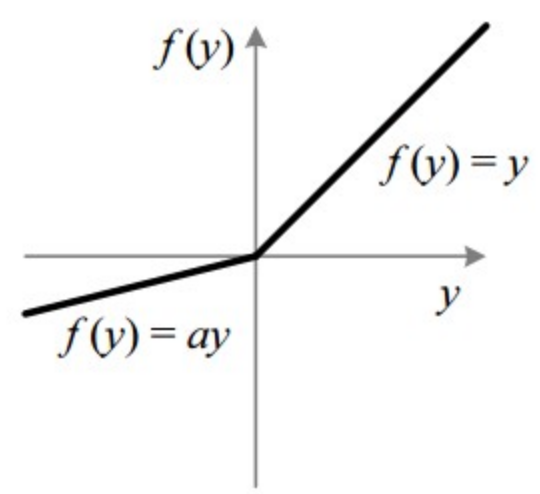
\includegraphics[width=0.3\textwidth]{img/lrelu}
     \caption{Função de Ativação \emph{Leaky ReLU}}
     \label{fig:lrelu}
\end{figure}

Na seção a seguir estão os resultados preliminares obtidos do treino dos modelos, hiperparâmetros e estratégias supracitados.
